% Options for packages loaded elsewhere
\PassOptionsToPackage{unicode}{hyperref}
\PassOptionsToPackage{hyphens}{url}
\PassOptionsToPackage{dvipsnames,svgnames,x11names}{xcolor}
\documentclass[
  10pt,
  fontset=fandol]{ctexart}
\usepackage{xcolor}
\usepackage[margin=16mm]{geometry}
\usepackage{amsmath,amssymb}
\setcounter{secnumdepth}{-\maxdimen} % remove section numbering
\usepackage{iftex}
\ifPDFTeX
  \usepackage[T1]{fontenc}
  \usepackage[utf8]{inputenc}
  \usepackage{textcomp} % provide euro and other symbols
\else % if luatex or xetex
  \usepackage{unicode-math} % this also loads fontspec
  \defaultfontfeatures{Scale=MatchLowercase}
  \defaultfontfeatures[\rmfamily]{Ligatures=TeX,Scale=1}
\fi
\usepackage{lmodern}
\ifPDFTeX\else
  % xetex/luatex font selection
\fi
% Use upquote if available, for straight quotes in verbatim environments
\IfFileExists{upquote.sty}{\usepackage{upquote}}{}
\IfFileExists{microtype.sty}{% use microtype if available
  \usepackage[]{microtype}
  \UseMicrotypeSet[protrusion]{basicmath} % disable protrusion for tt fonts
}{}
\makeatletter
\@ifundefined{KOMAClassName}{% if non-KOMA class
  \IfFileExists{parskip.sty}{%
    \usepackage{parskip}
  }{% else
    \setlength{\parindent}{0pt}
    \setlength{\parskip}{6pt plus 2pt minus 1pt}}
}{% if KOMA class
  \KOMAoptions{parskip=half}}
\makeatother
\usepackage{graphicx}
\makeatletter
\newsavebox\pandoc@box
\newcommand*\pandocbounded[1]{% scales image to fit in text height/width
  \sbox\pandoc@box{#1}%
  \Gscale@div\@tempa{\textheight}{\dimexpr\ht\pandoc@box+\dp\pandoc@box\relax}%
  \Gscale@div\@tempb{\linewidth}{\wd\pandoc@box}%
  \ifdim\@tempb\p@<\@tempa\p@\let\@tempa\@tempb\fi% select the smaller of both
  \ifdim\@tempa\p@<\p@\scalebox{\@tempa}{\usebox\pandoc@box}%
  \else\usebox{\pandoc@box}%
  \fi%
}
% Set default figure placement to htbp
\def\fps@figure{htbp}
\makeatother
\setlength{\emergencystretch}{3em} % prevent overfull lines
\providecommand{\tightlist}{%
  \setlength{\itemsep}{0pt}\setlength{\parskip}{0pt}}
\usepackage{amsmath,amssymb,mathtools,needspace}
\xeCJKDeclareCharClass{CJK}{"2032,"0400->"04FF,"2160->"216B,"2460->"2473,"25A0,"25C7,"25CB,"25CF}
\IfFontExistsTF{Arial Unicode MS}{\xeCJKsetup{AutoFallBack=true}\setCJKfallbackfamilyfont{\CJKrmdefault}{Arial Unicode MS}}{}
\setcounter{secnumdepth}{0}
\setlength{\emergencystretch}{2em}
\allowdisplaybreaks
\usepackage{bookmark}
\IfFileExists{xurl.sty}{\usepackage{xurl}}{} % add URL line breaks if available
\urlstyle{same}
\hypersetup{
  pdftitle={梯形格式},
  colorlinks=true,
  linkcolor={Maroon},
  filecolor={Maroon},
  citecolor={Blue},
  urlcolor={Blue},
  pdfcreator={LaTeX via pandoc}}

\title{梯形格式}
\author{}
\date{}

\begin{document}
\maketitle

\subsubsection{5.2.3 梯形格式}\label{ux68afux5f62ux683cux5f0f}

比较 Euler 格式与后退的 Euler 格式的误差公式 (5.2.3)、(5.2.7)，可以看到，如果将这两种方法进行算术平均，即可消除误差的主要部分 \(\pm\dfrac{h^2}{2}y''_n\) 而获得更高的精度。这种平均化方法通常称为\textbf{梯形方法}，其计算格式为

\[
y_{n+1}=y_n+\frac{h}{2}[f(x_n,y_n)+f(x_{n+1},y_{n+1})].\tag{5.2.8}
\]

梯形方法的这种平均化思想亦可借助于几何直观来说明，仍设顶点 \(P_n(x_n,y_n)\) 落在积分曲线 \(y=y(x)\) 上（见图 5.3），用 Euler 方法求解时，过点 \(P_n\) 以斜率 \(f(x_n,y_n)\) 引折线交 \(x=x_{n+1}\) 得出顶点 \(A\)，而用后退的 Euler 方法求解时，则以点 \(Q(x_{n+1},y_{n+1})\) 的斜率 \(f(x_{n+1},y_{n+1})\) 从顶点 \(P_n\) 引折线交 \(x=x_{n+1}\) 得另一顶点 \(B\)。\(A\) 和 \(B\) 两点均偏离

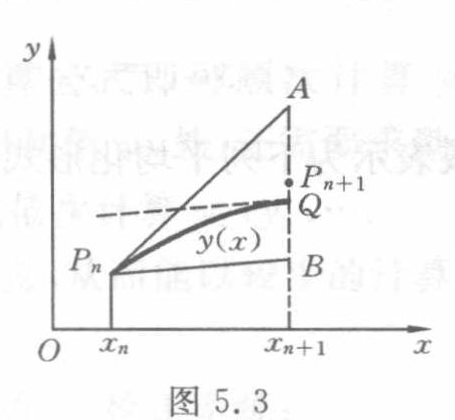
\includegraphics[width=0.85\linewidth,height=\textheight,keepaspectratio,alt={图 5.3 原图}]{../assets/ch05a/fig-5.3.png}

图 5.3（原图）：\(P_n\) 出发的两条线分别交 \(x=x_{n+1}\) 于 \(A,B\)，取平均所得点为 \(P_{n+1}\)；积分曲线标为 \(y(x)\)。原图全部标签：\(O,\allowbreak x,\allowbreak y,\allowbreak x_n,\allowbreak x_{n+1},\allowbreak P_n,\allowbreak A,\allowbreak B,\allowbreak P_{n+1},\allowbreak Q,\allowbreak y(x)\)。

\href{../../source-images/pdf-123.jpeg}{原页}

点 \(Q\) 比较远，然而从图形上可以明显地看出，\(AB\) 的中点 \(P_{n+1}\) 相当接近点 \(Q\)，可见梯形方法确实改善了精度（这里的解释不够严密，然而是令人信服的）。

梯形方法是隐式的，可用迭代法求解。同后退的 Euler 方法一样，仍用 Euler 方法提供迭代初值，则梯形法的迭代公式为

\[
\begin{cases}
y_{n+1}^{(0)}=y_n+hf(x_n,y_n),\\
y_{n+1}^{(k+1)}=y_n+\dfrac{h}{2}[f(x_n,y_n)+f(x_{n+1},y_{n+1}^{(k)})]
\end{cases}
\quad(k=0,1,2,\cdots).\tag{5.2.9}
\]

为了分析迭代过程的收敛性，将式 (5.2.8) 与式 (5.2.9) 相减，得

\[
y_{n+1}-y_{n+1}^{(k+1)}=\frac{h}{2}[f(x_{n+1},y_{n+1})-f(x_{n+1},y_{n+1}^{(k)})],
\]

于是有

\[
|y_{n+1}-y_{n+1}^{(k+1)}|\leqslant\frac{hL}{2}|y_{n+1}-y_{n+1}^{(k)}|,
\]

其中 \(L\) 为 \(f(x,y)\) 关于 \(y\) 的 Lipschitz 常数。如果选取 \(h\) 充分小，使得 \(\dfrac{hL}{2}<1\)，则当 \(k\to\infty\) 时有 \(y_{n+1}^{(k)}\to y_{n+1}\)，这说明迭代过程 (5.2.9) 是收敛的（关于迭代法的收敛性，可参见 6.2 节）。

\end{document}
